\documentclass[20pt]{beamer}
\mode<presentation>{\usetheme[green]{PosterWUR}}

\usepackage{fontspec}
\setsansfont{DejaVu Sans}
\usepackage[orientation=portrait,size=a0]{beamerposter}
\usepackage{tabularx, booktabs}
\usepackage{hyperref}
\usepackage{qrcode}
%\usepackage{caption}
%\usepackage{subcaption}
\newcolumntype{Y}{>{\centering\arraybackslash}X}

\TPGrid[30mm,30mm]{15}{25}  % 7 - 1 - 7 Columns

\usepackage{graphics}

\title{Comparison of machine learning algorithms for fuzzy land cover classification}
\author{Dainius Masiliūnas, Nandin-Erdene Tsendbazar, Jan Verbesselt}


\begin{document}
  \beamertemplatenavigationsymbolsempty
  \begin{frame}{} 

	\begin{textblock}{15}(12,3.8)
		
\includegraphics[height=0.5\TPVertModule]{figures/PVMEP.png} \hskip 1cm
		
\includegraphics[height=0.5\TPVertModule]{figures/vito-black}
	\end{textblock}

	\begin{textblock}{7}(0,4.9)
	  \Line
	  \LHead{1. Abstract}
	  The current standard of land cover classification is to assign each pixel to one land cover class, which at coarse resolution causes loss of information about mixed land cover. Fuzzy land cover classification, which assigns fractions of each land cover class to each pixel, can deal with mixed pixels. However, so far its application has been limited to city-scale areas and four or fewer classes.
	  
	  In this paper, the classification accuracy and processing speed were compared for three fuzzy classification machine learning algorithms: random forest regression, fuzzy \textit{c}-means, neural networks. The algorithms were used to classify the whole boreal-temperate forest gradient zone between Finland and Lithuania into nine land cover classes. Results showed that all of the tested algorithms are able to achieve similarly high classification accuracy. Random forest regression accuracy was the highest, but its processing speed was the lowest. The results are a milestone for creating a global fuzzy land cover classification product incorporating user-specific requirements.
	
	\end{textblock}
	
	\begin{textblock}{7}(0,10)
	  \Line 
	  \LHead{2. Data and methods}
	  6 spectral and 4 temporal metrics were derived from the full 100 m Proba-V surface reflectance archive over tile X20Y01. EUDEM was used to derive 4 terrestrial metrics. These metrics (see figure \ref{fig-varimp}) were input into machine learning models (fuzzy \textit{c}-means, random forest regression, neural networks) for predicting the fraction of each land cover class in each pixel: cultivated land, deciduous trees, evergreen trees, shrubs, grasslands, barren, wetland, built-up and water. The models were trained and validated on samples collected through manual high-resolution image interpretation. All processing was done on a virtual machine with 32 threads and 32 GiB RAM.
	  
	  \begin{figure}
			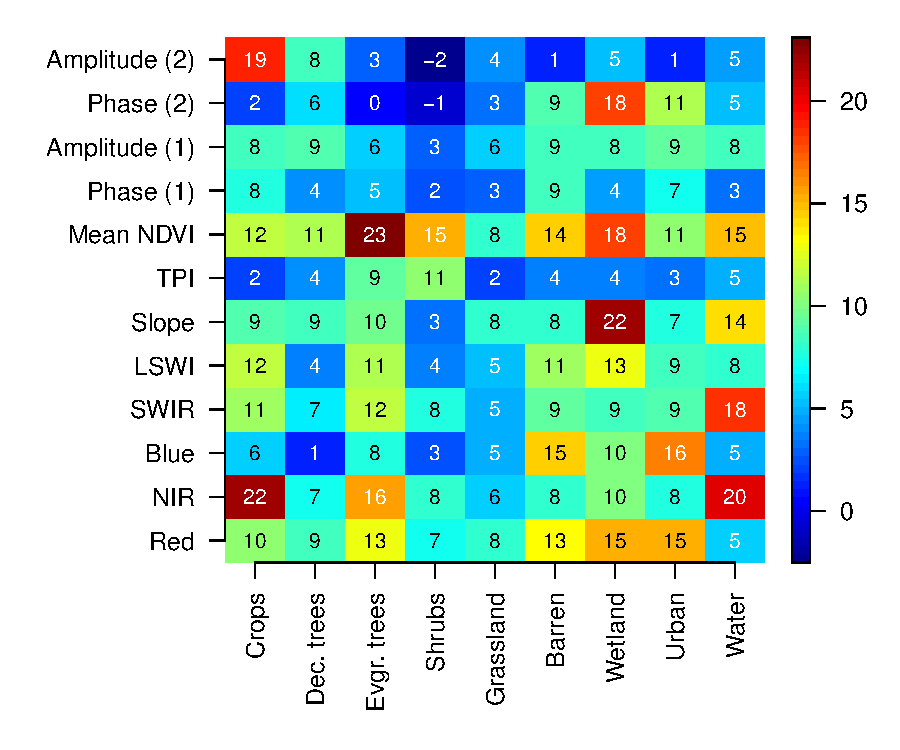
\includegraphics[width=7\TPHorizModule]{../thesis/thesis-figures/variable-importance}
			\caption{Covariate permutation importance for holdout random forest regression. X axis: all covariates used in this study, Y axis: all classes used in this study. Values indicate the increase in prediction RMSE when a given covariate is shuffled: higher values mean higher importance of the covariate.}
			\label{fig-varimp}
      \end{figure}
	
	\end{textblock}
	
	\begin{textblock}{7}(8,4.9)
		\Line
		\LHead{3. Results}
		
		\begin{figure}
		  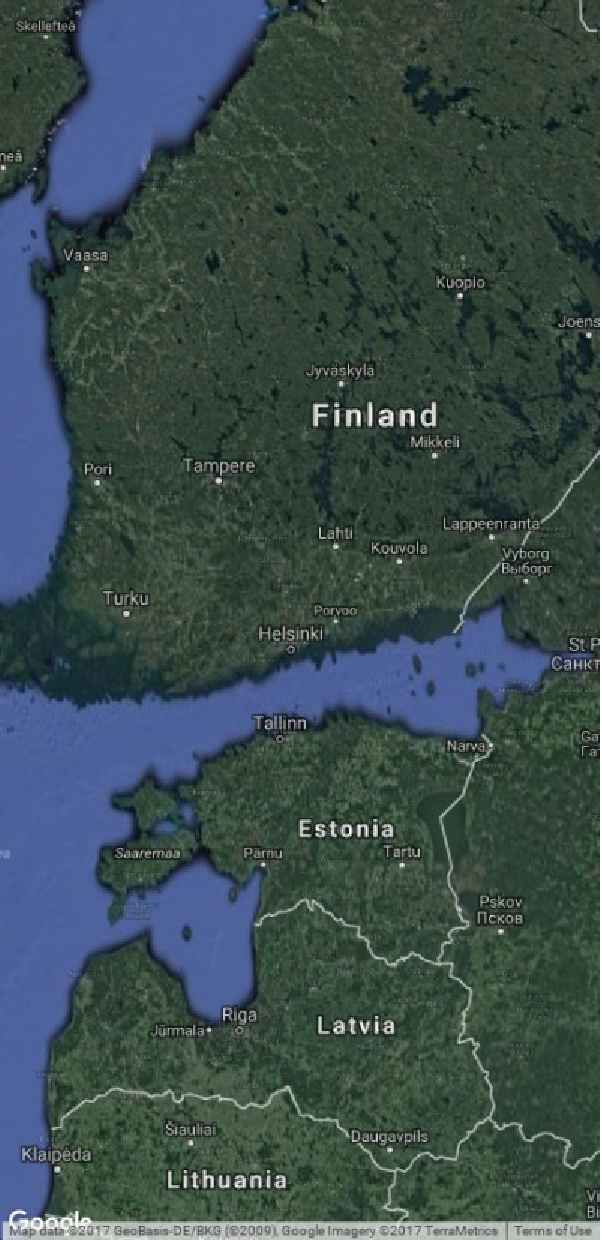
\includegraphics[width=2.3\TPHorizModule]{../thesis/thesis-figures/figures-qgis/fulltile-google}
		  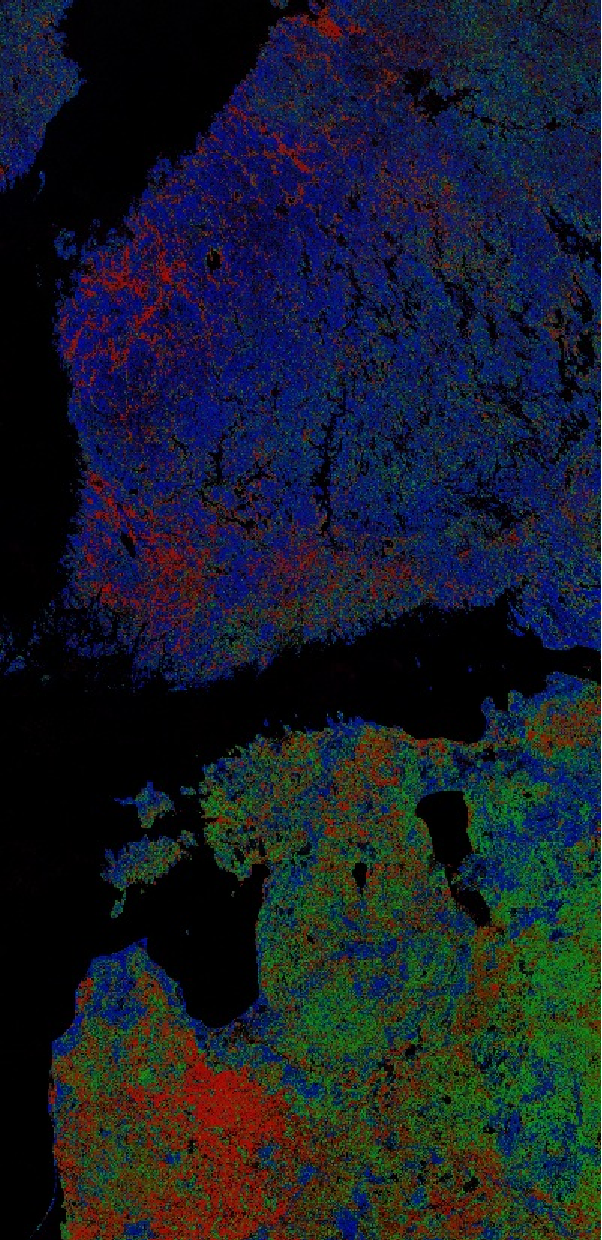
\includegraphics[width=2.3\TPHorizModule]{../thesis/thesis-figures/figures-qgis/fulltile-rf}
		  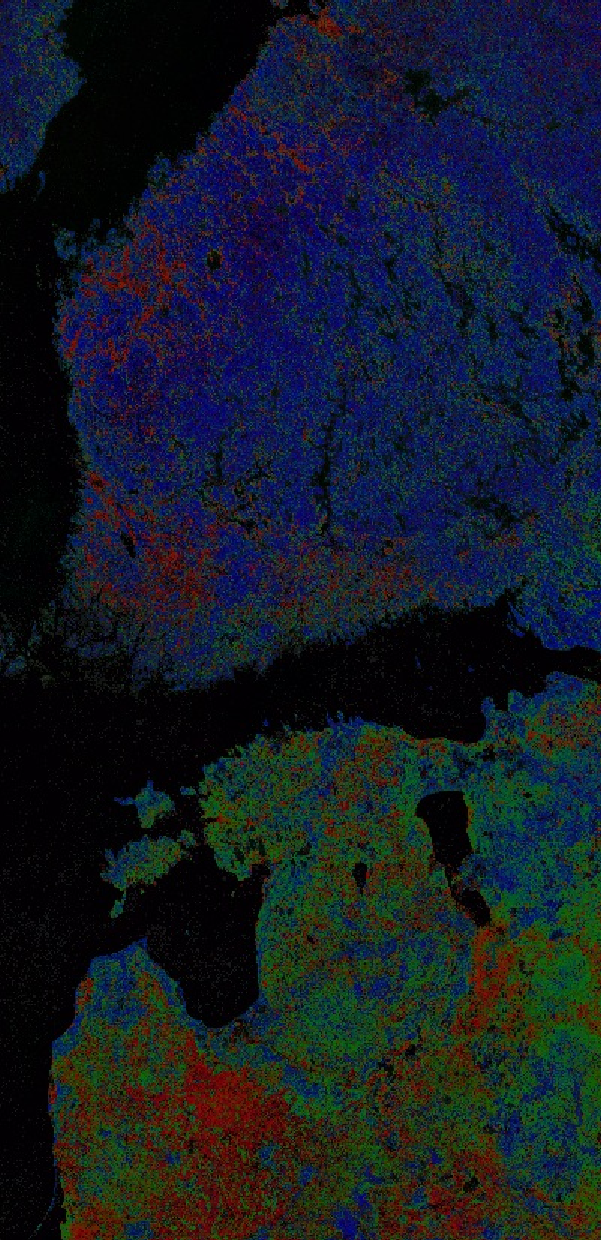
\includegraphics[width=2.3\TPHorizModule]{../thesis/thesis-figures/figures-qgis/fulltile-nn}
		  \caption{Results of full-tile fuzzy classification. Left: true colour Google imagery of the study area; middle: random forest regression algorithm; right: neural network algorithm. The colours represent classes: cultivated land (red), deciduous trees (green), evergreen trees (blue).}
		\end{figure}
		
		\begin{figure}
		  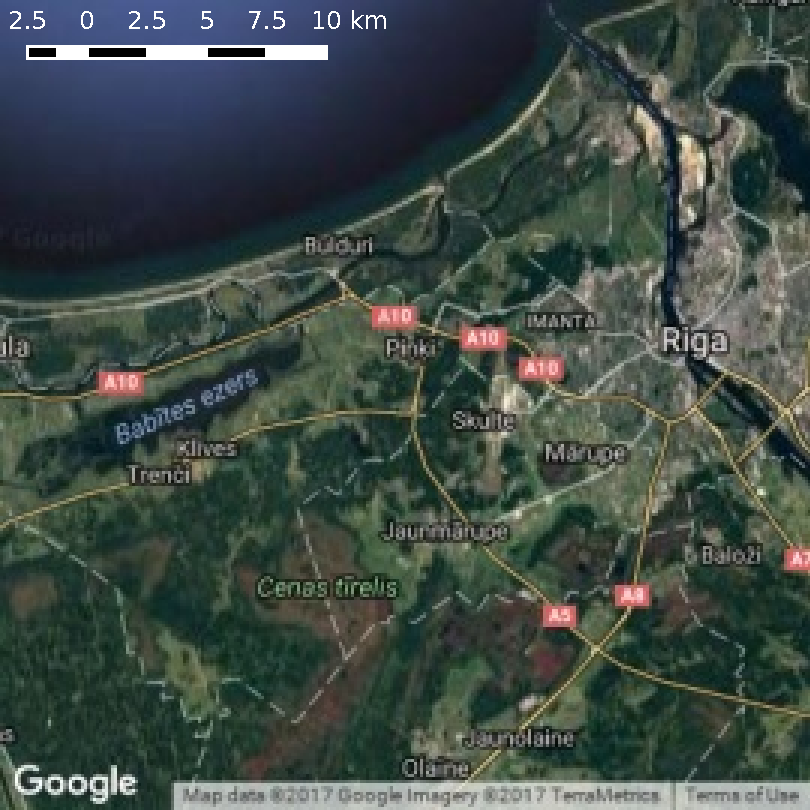
\includegraphics[width=2.3\TPHorizModule]{../thesis/thesis-figures/figures-qgis/riga-google}
		  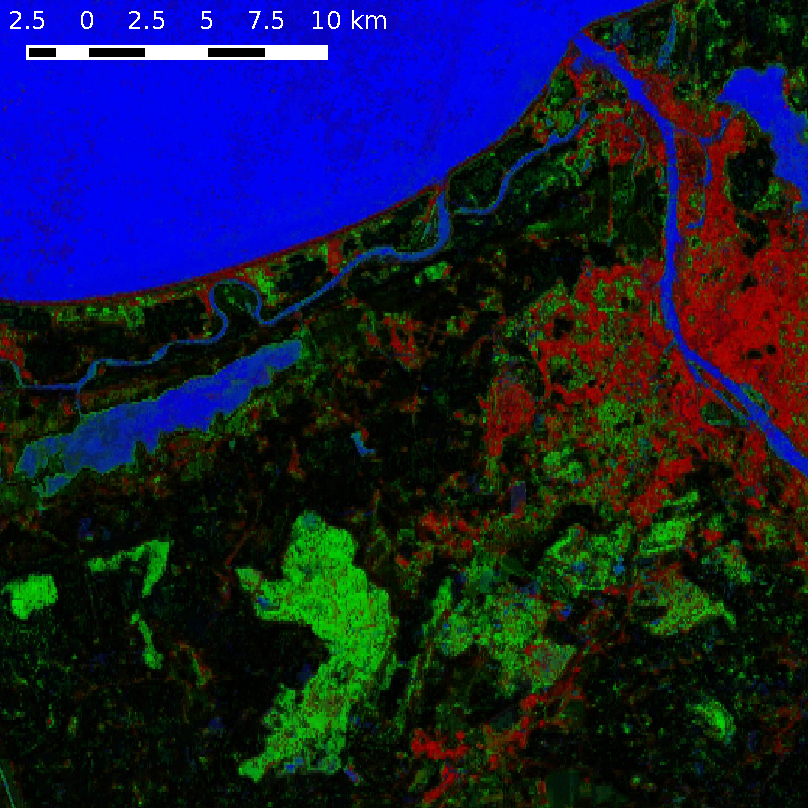
\includegraphics[width=2.3\TPHorizModule]{../thesis/thesis-figures/figures-qgis/riga-rf}
		  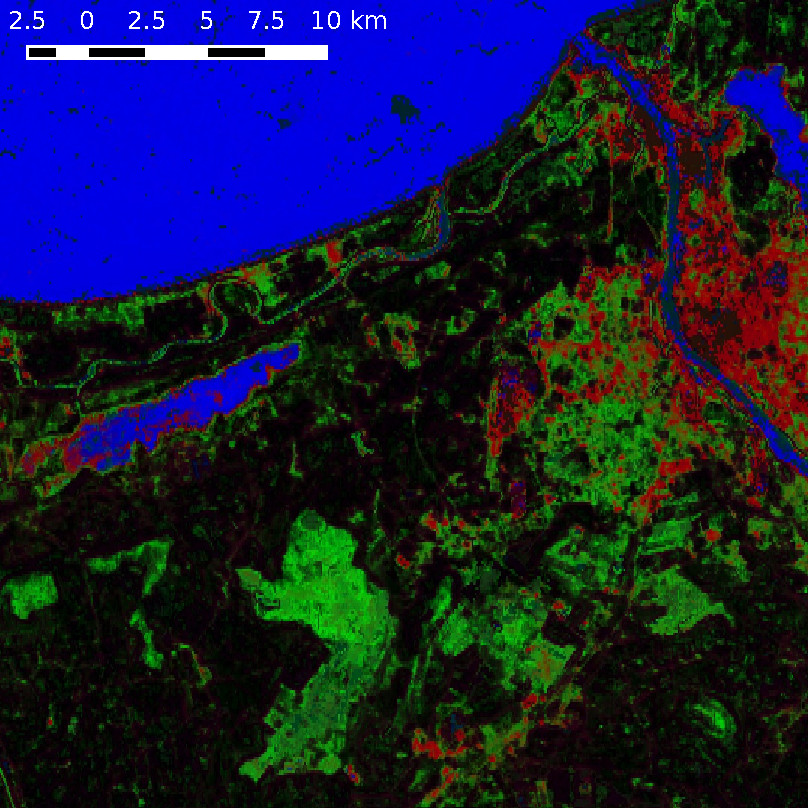
\includegraphics[width=2.3\TPHorizModule]{../thesis/thesis-figures/figures-qgis/riga-nn}
		  \caption{Close-up of fuzzy classification in the area surrounding the city of Rīga, Latvia. Left: true colour Google imagery; middle: random forest regression algorithm; right: neural network algorithm. The colours represent classes: built-up (red), wetlands (green), water (blue).}
		\end{figure}



	\end{textblock}
	
	\begin{textblock}{7}(8,16.7)
		\Line
		\LHead{4. Conclusion}
		Random forest regression was the most accurate (MAE: 11.7\%), but not significantly more than fuzzy \textit{c}-means (MAE: 12.0\%) and neural networks (MAE: 12.7\%). The prediction times were very different: 1229, 42 and 25 minutes respectively to process an entire tile. Thus random forest regression was the most accurate but slowest algorithm, neural networks was the least accurate and fastest. All of these algorithms produced spatially consistent output. All types of covariates were important to include in the models, with the exception of terrain aspect and the Proba-V water mask (see figure \ref{fig-varimp}).
		
		%\begin{table}
		%	\caption{This is a table}
		%	\begin{tabularx}{\textwidth}{c *{6}{Y}}
		%	\toprule
		%	Foo bar
		%	 & \multicolumn{3}{c}{Fantastical aardvarks}  
		%	 & \multicolumn{3}{c}{Spelunking elephants}\\
		%	\cmidrule(lr){2-4} \cmidrule(l){5-7}
		%	  & A & B & C & A & B & C\\
		%	\midrule
		%	 5  & 87 &  5 &  2 & 82 & 18 & 48\\
		%	 6  &  5 & 43 &  4 &  7 & 47 &  4\\
		%	 7  &  7 & 18 & 63 &  2 &  9 & 99\\
		%	\bottomrule
		%	\end{tabularx}	
		%\end{table}	

	\end{textblock}

	\begin{textblock}{7}(8,19.9)
		\Line
		\LHead{5. Discussion}
		Fractional land cover mapping is capable of representing smooth transitions between classes in space (and time), and users can produce customised discrete maps by defining their own rules. Larger scale application of fuzzy classification is needed to test whether it is computationally feasible for global mapping and whether model accuracies change depending on the area of interest.
		
	\end{textblock}
	
	\begin{textblock}{7}(0,21.5)
		\Line
		\LHead{6. Acknowledgements}
		We would like to thank VITO for providing access to and support for computational resources on the Proba-V Mission Exploitation Platform (MEP).
		
	\end{textblock}
	
	%\begin{textblock}{7}(8,21)
	%	\Line
	%	\LHead{Acknowledgements}
	%\end{textblock}

	\begin{textblock}{15}(0,23)
		\Line
	\end{textblock}	
	
	\begin{textblock}{1}(0,23.5)
		%\begin{figure}
		%\resizebox{1\TPHorizModule}{!}{
		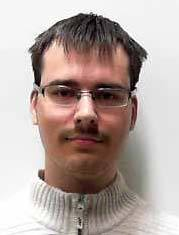
\includegraphics[height=1\TPHorizModule]{figures/dainius.jpeg}
		%} 
		%\end{figure} 
	\end{textblock}
	
	\begin{textblock}{7}(1,23.5)
		%\Adress{
		\small{\color{wursignblue}
            Dainius Masiliūnas\\
			Email: \url{dainius.masiliunas@wur.nl}\\
			LinkedIn: \url{https://www.linkedin.com/in/greatemerald} \\
			ResearchGate: \url{https://www.researchgate.net/profile/Dainius_Masiliunas} \\
			Laboratory of Geo-information Science and Remote Sensing, \url{http://www.wur.nl/grs}\\
			P.O. Box 47, 6700 AA Wageningen
		}
	\end{textblock}
	
	\begin{textblock}{5}(8,23.5)
        Read full text online: \\ \url{https://edepot.wur.nl/424175} \\
        Source code: \\ \url{https://github.com/GreatEmerald/master-classification}
	\end{textblock}
	
	\begin{textblock}{2}(13.5,23.5)
        \qrcode[height=7.5cm]{https://edepot.wur.nl/424175}
	\end{textblock}


  \end{frame}
\end{document}
